% 多源信息核验助手 — 介绍 PPT
% 编译(一次通过):  xelatex slides.tex   或   latexmk -xelatex slides.tex
% 依赖:beamer + xeCJK + Noto CJK 字体 + tikz(mindmap)
\documentclass[aspectratio=169,11pt]{beamer}

\usepackage{xeCJK}
\setCJKmainfont{Noto Serif CJK SC}
\setCJKsansfont{Noto Sans CJK SC}
\setCJKmonofont{Noto Sans Mono CJK SC}
\usepackage{fontspec}

\usepackage{tikz}
\usetikzlibrary{mindmap,trees,arrows.meta,positioning,shapes.geometric,backgrounds,fit}
\usepackage{booktabs}

\usetheme{default}
\useinnertheme{circles}
\setbeamertemplate{navigation symbols}{}
\setbeamertemplate{footline}[frame number]

% --- palette ---
\definecolor{ink}{HTML}{0F172A}
\definecolor{indigo}{HTML}{4F46E5}
\definecolor{sky}{HTML}{0EA5E9}
\definecolor{teal}{HTML}{14B8A6}
\definecolor{amber}{HTML}{F59E0B}
\definecolor{rose}{HTML}{EF4444}
\definecolor{green}{HTML}{22C55E}
\definecolor{violet}{HTML}{A855F7}
\definecolor{slate}{HTML}{64748B}
\definecolor{paper}{HTML}{F8FAFC}

\setbeamercolor{frametitle}{fg=white,bg=indigo}
\setbeamercolor{title}{fg=ink}
\setbeamercolor{structure}{fg=indigo}
\setbeamercolor{normal text}{fg=ink}
\setbeamerfont{frametitle}{series=\bfseries}

\title{\textbf{多源信息核验助手}}
\subtitle{Multi-source Information Verification Assistant}
\author{中国科学院软件研究所 · 中文信息处理实验室 Coding 测试 — 任务3}
\date{}

% 小工具:阶段色块
\newcommand{\stage}[2]{\tikz[baseline]{\node[fill=#1,text=white,rounded corners=2pt,inner sep=2pt,font=\scriptsize\bfseries]{#2};}}

\begin{document}

% ---------- 1. 封面 ----------
\begin{frame}[plain]
  \centering
  \vfill
  {\Huge\bfseries\color{indigo} 多源信息核验助手}\\[2mm]
  {\large Multi-source Information Verification Assistant}\\[6mm]
  \begin{tikzpicture}
    \foreach \c/\t [count=\i] in {indigo/抽取断言, sky/多源检索, teal/证据研判, amber/可信度评分, green/带引用报告}{
      \node[fill=\c,text=white,rounded corners=3pt,minimum height=7mm,inner xsep=6pt,font=\small\bfseries] at (\i*2.7,0) {\t};
      \ifnum\i<5 \draw[-{Latex},thick,slate] (\i*2.7+0.95,0)--(\i*2.7+1.75,0);\fi
    }
  \end{tikzpicture}\\[8mm]
  {\color{slate} 输入一段说法,系统自动核验其真伪、给出依据与可信度}\\[6mm]
  {\footnotesize\color{slate} 中国科学院软件研究所 · 中文信息处理实验室 Coding 测试 — 任务3}
  \vfill
\end{frame}

% ---------- 2. 问题与设计哲学 ----------
\begin{frame}{为什么"让大模型判断对错"不够 —— 问题分析}
  \begin{columns}[T]
    \begin{column}{0.5\textwidth}
      \textbf{自动核验的四个本质难点:}
      \begin{enumerate}\setlength\itemsep{4pt}
        \item \textbf{断言不是句子}:一句话常含多个事实点,不拆开无法定位错误。
        \item \textbf{LLM 的"知道"不可信、不可追溯}:证据必须来自模型之外、可点击核对的来源。
        \item \textbf{证据有好坏}:同行评审 / 预印本 / 百科 / 网页可信度迥异,旧结论可能已被推翻。
        \item \textbf{要有"不确定"档}:大量断言是证据不足或来源矛盾。
      \end{enumerate}
    \end{column}
    \begin{column}{0.5\textwidth}
      \textbf{设计哲学:把人类核查流程显式化}
      \vspace{2mm}
      \footnotesize
      \begin{tabular}{@{}l@{\;}c@{\;}l@{}}
        \textit{人类核查者} & & \textit{系统阶段}\\\midrule
        在主张什么? & $\to$ & \stage{indigo}{①断言抽取}\\[3pt]
        去哪查、查什么? & $\to$ & \stage{sky}{②检索规划}\\[3pt]
        翻资料 & $\to$ & \stage{teal}{③多源检索}\\[3pt]
        支持还是反对?可信吗? & $\to$ & \stage{amber}{④证据研判}\\[3pt]
        有多少把握? & $\to$ & \stage{violet}{⑤裁决聚合}\\[3pt]
        写带引用的结论 & $\to$ & \stage{green}{⑥生成报告}\\
      \end{tabular}
      \vspace{3mm}
      \scriptsize\color{slate} 核心信念:不用一次 LLM 调用替代整个核查过程;每步只让模型做它擅长的语言判断。
    \end{column}
  \end{columns}
\end{frame}

% ---------- 3. 系统架构 ----------
\begin{frame}{系统架构 —— 六阶段异步流水线 + 流式可观测}
  \centering
  \resizebox{\textwidth}{!}{%
  \begin{tikzpicture}[font=\footnotesize,node distance=6mm,
      box/.style={rounded corners=3pt,minimum height=11mm,minimum width=26mm,text=white,align=center,font=\bfseries},
      io/.style={draw=slate,thick,rounded corners=3pt,minimum height=11mm,minimum width=24mm,align=center}]
    \node[io] (in) {文本 / URL / 文件\\\scriptsize inputs 归一化};
    \node[box,fill=indigo,right=of in] (c1) {①断言抽取};
    \node[box,fill=sky,right=of c1] (c2) {②检索规划\\\scriptsize +路由};
    \node[box,fill=teal,right=of c2] (c3) {③多源检索\\\scriptsize 并发+去重};
    \node[box,fill=amber,right=of c3] (c4) {④证据研判};
    \node[box,fill=violet,right=of c4] (c5) {⑤裁决聚合\\\scriptsize 可信度评分};
    \node[box,fill=green,right=of c5] (c6) {⑥生成报告\\\scriptsize 编号引用};
    \foreach \a/\b in {in/c1,c1/c2,c2/c3,c3/c4,c4/c5,c5/c6}{
      \draw[-{Latex},thick] (\a)--(\b);}
    \begin{scope}[on background layer]
      \node[draw=slate,dashed,rounded corners,fit=(c1)(c6),inner sep=3.5mm,
        label={[slate]above:\,pipeline.py 编排,每步 emit 事件 → SSE 推送前端\,}] {};
    \end{scope}
  \end{tikzpicture}}
  \vspace{4mm}
  \resizebox{\textwidth}{!}{%
  \begin{tikzpicture}[font=\footnotesize,chip/.style={text=white,rounded corners=3pt,minimum height=8mm,inner xsep=7pt,font=\bfseries}]
    \node[font=\bfseries] (lbl) {可插拔证据源(统一 \texttt{Source} 接口,均无需 API key):};
    \node[chip,fill=teal,right=3mm of lbl] (s1) {Wikipedia};
    \node[chip,fill=indigo,right=2mm of s1] (s2) {arXiv};
    \node[chip,fill=sky,right=2mm of s2] (s3) {Semantic Scholar};
    \node[chip,fill=violet,right=2mm of s3] (s4) {Crossref};
    \node[chip,fill=slate,right=2mm of s4] (s5) {Web};
  \end{tikzpicture}}
  \vspace{3mm}
  {\footnotesize 全异步并发(断言之间、源×查询之间);单源失败被吞掉,不拖垮整体。}
\end{frame}

% ---------- 4. 思维导图:能力全景 ----------
\begin{frame}{能力全景(思维导图)}
  \centering
  \begin{tikzpicture}[
      mindmap, % 保留此选项以保持节点外观风格
      every node/.style={concept, concept color=indigo!70, text=white, font=\tiny, rotate=0, minimum size=1.5cm},
 % 全局强制文字不旋转
      level 1/.append style={level distance=3.4cm}, % 一级节点距离
      level 2/.append style={level distance=2.2cm}, % 二级节点距离
      scale=0.6, transform shape
    ]
\begin{scope}[on background layer]
    \node[font=\normalsize]{核验\\助手}
      % 一级节点：手动指定 grow 角度 (360/5 = 72度间隔，从90度开始)
      child[grow=90, concept color=sky]{ 
        node[font=\footnotesize]{输入} 
        % 二级节点：围绕父节点继续放射
        child[grow=150]{node{文本}} 
        child[grow=120]{node{URL}} 
        child[grow=90]{node{文件}} 
      }
      child[grow=18, concept color=teal]{ 
        node[font=\footnotesize]{多源\\证据} 
        child[grow=78]{node{学术\\库}} 
        child[grow=48]{node{百科}} 
        child[grow=18]{node{网页}} 
      }
      child[grow=306, concept color=amber, font=\normalsize]{ 
        node[font=\footnotesize]{评估} 
        child[grow=336]{node{立场}} 
        child[grow=306]{node{质量}} 
        child[grow=276]{node{时效}} 
      }
      child[grow=234, concept color=violet, font=\normalsize]{ 
        node[font=\footnotesize]{裁决} 
        child[grow=264]{node{五档}} 
        child[grow=234]{node{可信\\度}} 
        child[grow=204]{node{冲突}} 
      }
      child[grow=162, concept color=green, font=\normalsize]{ 
        node[font=\footnotesize]{产出} 
        child[grow=192]{node{引用\\报告}} 
        child[grow=162]{node{实时\\轨迹}} 
        child[grow=132]{node{反馈}} 
      };
\end{scope}
  \end{tikzpicture}
\end{frame}

% ---------- 5. 设计亮点1:人机分工 + 评分公式 ----------
\begin{frame}{设计亮点 ① —— 人机分工 + 可审计的可信度评分}
  \begin{columns}[T]
    \begin{column}{0.52\textwidth}
      \textbf{评估证据 = LLM 判语义 ⊕ 代码算分数}
      \begin{itemize}\footnotesize
        \item \textbf{LLM 做擅长的}:立场(支持/反驳/中立)、相关性、置信度、一句话理由(一次批量判完)。
        \item \textbf{代码做该确定的}:来源\textbf{质量}(同行评审 0.85 > 百科 0.70 > 预印本 0.60 > 网页 0.40)、\textbf{时效}(20年窗口衰减、设 0.3 下限保护经典文献)。
      \end{itemize}
      \vspace{1mm}
      {\scriptsize\color{slate} 打分可复现、可审计、可解释——不是黑箱数字。}
      \vspace{2mm}
      \footnotesize
      $$\text{weight}=\text{rel}\times\text{qual}\times(0.6{+}0.4\,\text{rec})\times\text{conf}$$
    \end{column}
    \begin{column}{0.48\textwidth}
      \textbf{可信度 = 方向 × 强度}
      \vspace{1mm}
      \footnotesize
      \[ \text{ratio}=\frac{w_{\text{支持}}}{w_{\text{支持}}+w_{\text{反驳}}} \]
      \[ \text{strength}=\min\!\Big(1,\tfrac{w_{\text{总}}}{w_{\text{ref}}}\Big) \]
      \[ \boxed{\,\text{cred}=50+(\text{ratio}{-}0.5)\times100\times\text{strength}\,} \]
      \vspace{1mm}
      \begin{itemize}\scriptsize
        \item 弱/少证据 $\Rightarrow$ strength 小 $\Rightarrow$ 分数停在 50(不确定)。
        \item 多个强一致来源 $\Rightarrow$ 决定性推向 0 或 100。
        \item "证据不足"自然落在 50,而非被误判真/假。
      \end{itemize}
    \end{column}
  \end{columns}
\end{frame}

% ---------- 6. 设计亮点2:五档裁决 + 冲突 ----------
\begin{frame}{设计亮点 ② —— 五档裁决、诚实地暴露分歧}
  \centering
  \begin{tikzpicture}[font=\small,node distance=3mm]
    \foreach \c/\t [count=\i] in {green/证据支持, rose/证据反驳, amber/部分支持, violet/证据冲突, slate/证据不足}{
      \node[fill=\c,text=white,rounded corners=3pt,minimum height=8mm,inner xsep=8pt,font=\bfseries] at (\i*2.6,0) {\t};
    }
  \end{tikzpicture}
  \vspace{4mm}
  \begin{columns}[T]
    \begin{column}{0.5\textwidth}
      \textbf{证据冲突(conflicting)}
      \footnotesize
      \begin{itemize}
        \item 当支持与反驳权重都不可忽略,显式标注"高质量来源互相矛盾,需人工判读"。
        \item 前端用\textbf{支持 / 反驳 / 中立 三栏}对照可视化。
      \end{itemize}
    \end{column}
    \begin{column}{0.5\textwidth}
      \textbf{可插拔证据源}
      \footnotesize
      \begin{itemize}
        \item 统一 \texttt{Source} 协议,注册表加一行即接入新源。
        \item 按断言类型路由:研究结论→学术库;定义→百科;通用→网页。
        \item 查询刻意含"找反面证据"角度,抑制确认偏误。
      \end{itemize}
    \end{column}
  \end{columns}
\end{frame}

% ---------- 7. 工程实现 ----------
\begin{frame}{工程实现要点}
  \footnotesize
  \begin{tabular}{@{}p{3.1cm}p{8.4cm}@{}}
    \toprule
    \textbf{结构化 LLM 输出} & 用 \texttt{tool\_choice} 强制工具调用,入参即 JSON Schema,不合规自动重试——不靠"请输出 JSON"祈祷。\\
    \textbf{全异步并发} & 断言之间、(源×查询)之间 \texttt{asyncio} 并发 + 信号量限流;总耗时≈最慢单链路。\\
    \textbf{流式可观测} & 每阶段 \texttt{emit} 结构化事件,SSE 实时推前端(Agent 执行轨迹 = 可解释性)。\\
    \textbf{容错降级} & 单源/单查询失败被吞;Semantic Scholar 429 退避后降级返回空,不拖垮流水线。\\
    \textbf{多输入} & 文本 / URL(抓正文)/ 文件,按 content-type 分流。\\
    \textbf{反馈闭环} & \texttt{/api/feedback} 记录 👍/👎,为来源权重 / prompt 调优留接口。\\
    \bottomrule
  \end{tabular}
  \vspace{2mm}
  \\{\scriptsize 栈:FastAPI + httpx(全异步)· React + Vite + TS · Anthropic Claude · Docker 一键运行}
\end{frame}

% ---------- 8. 迭代过程(必备页) ----------
\begin{frame}{迭代过程 —— 真实开发记录(踩坑 → 修正)}
  \footnotesize
  \begin{tabular}{@{}cp{4.2cm}p{6.0cm}@{}}
    \toprule
    \# & \textbf{问题} & \textbf{修正} \\\midrule
    1 & 模型调用 400:\texttt{temperature} 已弃用 & 抓响应体定位,移除该参数;\textit{先用最小请求探活}\\
    2 & \texttt{/verify} 同时声明 JSON body 与 Form,JSON 被当表单 & 改读原始 Request,按 content-type 手动分流\\
    3 & DuckDuckGo POST 返回 202 挑战页、无结果 & 实测改用 GET 拿无 JS 结果页,解码 \texttt{uddg} 链接\\
    4 & Semantic Scholar 无 key 共享池偶发 429 & 指数退避重试 + 失败降级返回空\\
    5 & 时效直接相乘,压低经典论文(如 2017 Transformer) & 改用 $0.6{+}0.4\,\text{rec}$ 阻尼 + 0.3 下限\\
    6 & 需验证"子句级错误"能否被定位 & 用爱因斯坦例子验证:正确判出错误子句\\
    \bottomrule
  \end{tabular}
  \vspace{2mm}
  \\{\scriptsize 完整交互轨迹见仓库 \texttt{trace/}(Claude Code 会话记录)。}
\end{frame}

% ---------- 9. Demo 效果 ----------
\begin{frame}{Demo —— 它真的能定位到子句级别的错误}
  \begin{columns}[T]
    \begin{column}{0.46\textwidth}
      \textbf{输入}
      \vspace{1mm}
      \footnotesize\color{ink}
      ``爱因斯坦于 1921 年因\textbf{相对论}获得诺贝尔物理学奖。''
      \vspace{3mm}
      \\\textbf{系统输出}
      \begin{itemize}\footnotesize
        \item 拆成两条断言:\stage{green}{1921 年获诺奖}、\stage{rose}{因相对论获奖}
        \item 后者被判\textbf{证据反驳(0/100)}——实际因\textbf{光电效应}获奖。
        \item 整体可信度 $\approx$ \textbf{27/100},附 Wikipedia / 学术来源引用。
      \end{itemize}
      \vspace{2mm}
      {\scriptsize\color{slate} 这正是断言级拆分的价值:整句"看起来对",错误藏在子句里。}
    \end{column}
    \begin{column}{0.54\textwidth}
      \centering
      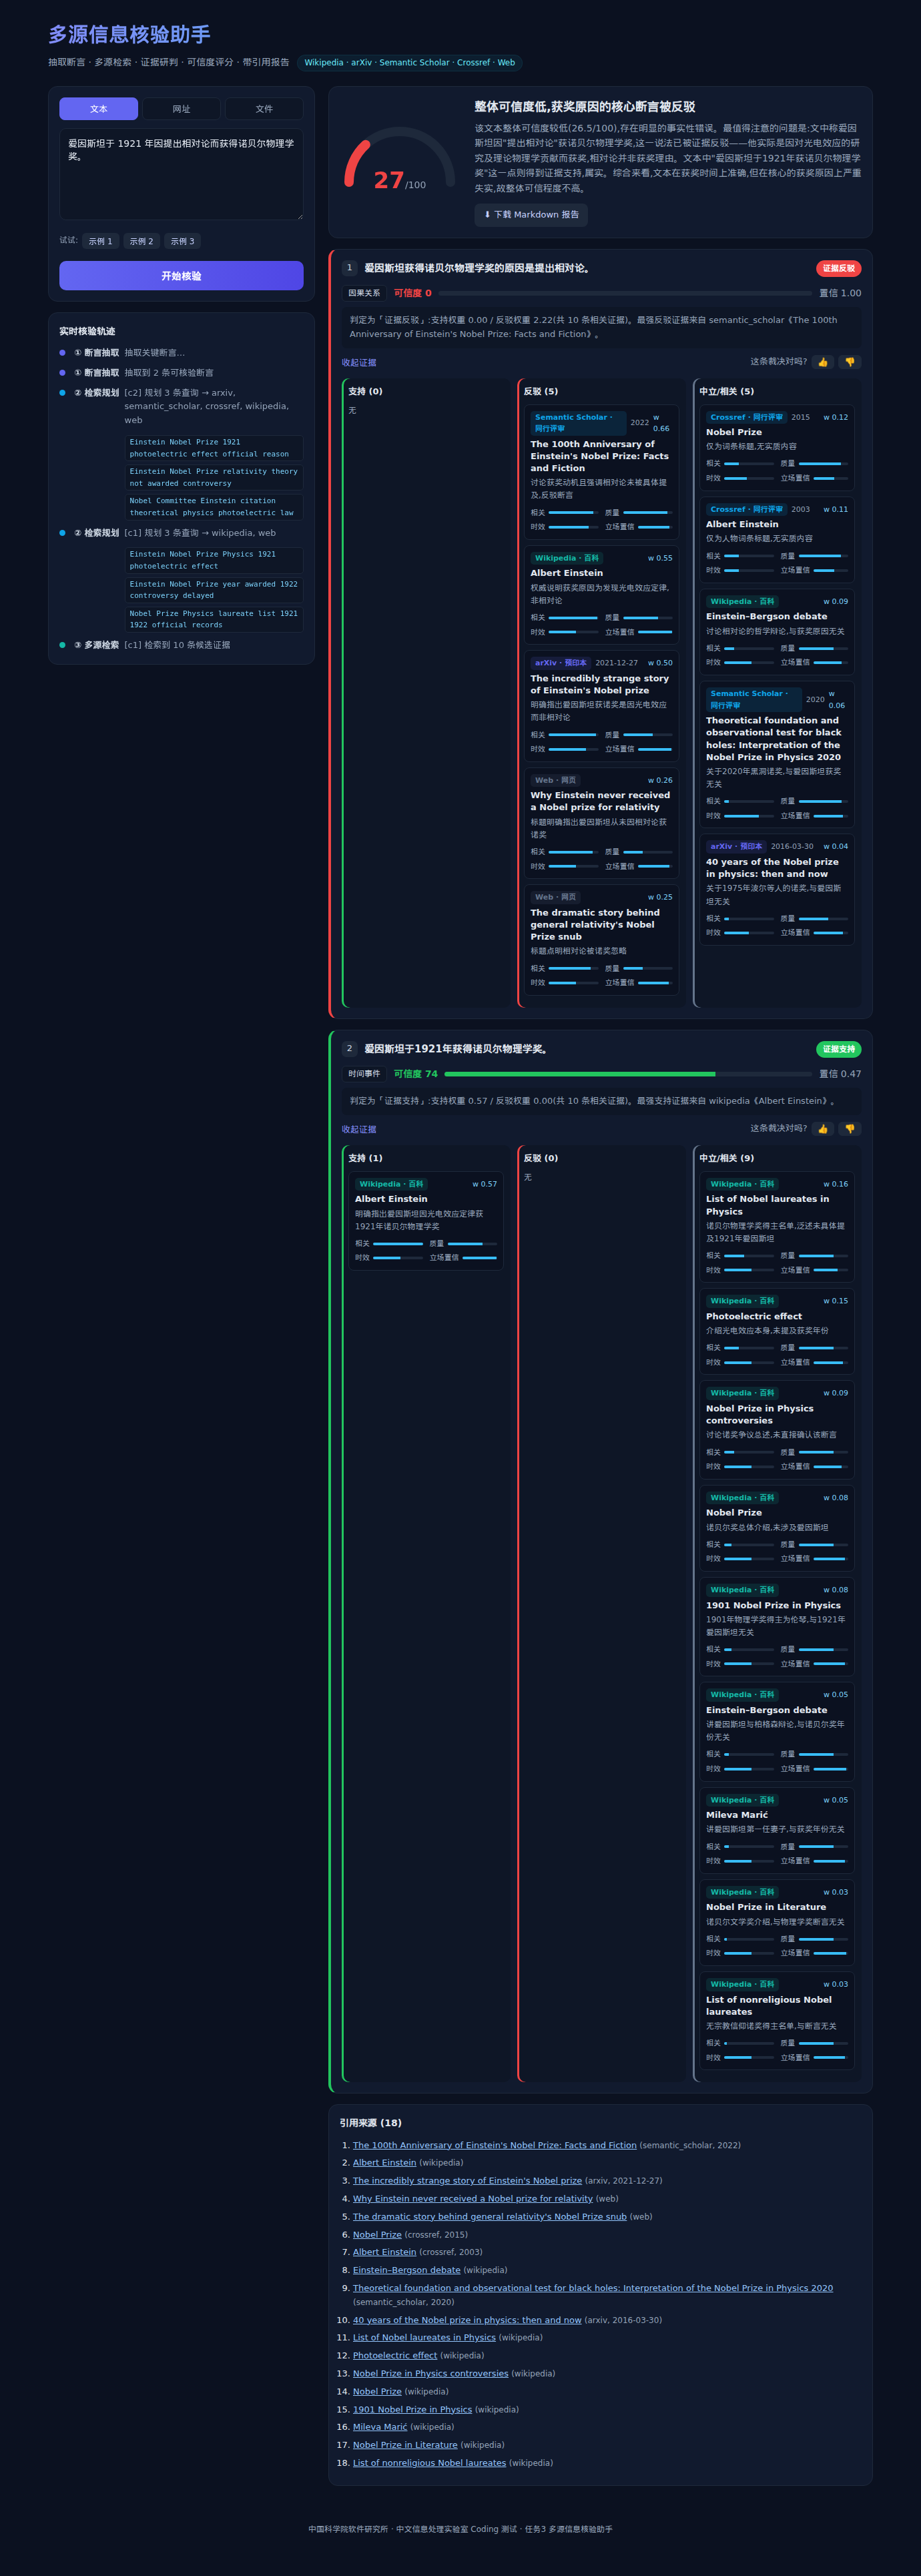
\includegraphics[width=\linewidth,height=0.78\textheight,keepaspectratio]{assets/demo-full.png}
    \end{column}
  \end{columns}
\end{frame}

% ---------- 10. 总结 ----------
\begin{frame}{总结 · 局限 · 未来}
  \begin{columns}[T]
    \begin{column}{0.5\textwidth}
      \textbf{已交付}
      \footnotesize
      \begin{itemize}
        \item 六阶段可解释核验流水线 + 五档裁决 + 可信度评分
        \item 5 个免费多源证据 adapter,按类型路由
        \item SSE 实时轨迹 + 冲突三栏可视化 + 带引用报告
        \item 多输入 / 反馈闭环 / Docker 一键运行
      \end{itemize}
    \end{column}
    \begin{column}{0.5\textwidth}
      \textbf{局限与未来}
      \footnotesize
      \begin{itemize}
        \item 用摘要判立场,未抓全文 → 段落级证据定位
        \item 中文证据源偏少 → 接入中文百科/知网
        \item 阈值为经验值 → 用标注数据集校准
        \item 反馈目前仅记录 → 在线调来源权重与策略
      \end{itemize}
    \end{column}
  \end{columns}
  \vfill
  \centering {\large\color{indigo}\bfseries 谢谢!}\\
  {\scriptsize\color{slate} 代码 · 设计文档 · 交互轨迹见仓库}
\end{frame}

\end{document}

编译后思维导图显示不全，帮我修复